\graphicspath{{images/}}

\section{\thesection~Methods}
\label{sec:methods}

\subsection{CANS}

To analyse QFA data using the competition model I developed the Python
package CANS which can be used for model composition, model
simulation, parameter inference, and visualisation of results. CANS
accepts cell density timecourses for any size rectangular array. CANS
can produce SBML models to document results of parameter inference or
for independent validation. It is relatively simple to create and
simulate new models involving reactions between species within
cultures or between neighbouring cultures, and to fit these provided
an initial guess. The CANS package is available at
\href{https://github.com/lwlss/CANS}{https://github.com/lwlss/CANS}.

\subsection{\thesubsection~Solving and fitting}

\subsubsection{Solving}

% [Only keep if I remove the CANS overview above: To analyse QFA data I
% created a Python package (``CANS'') for model composition, model
% simulation, parameter inference, and visualisation of results. CANS
% accepts timecourse data of cell density for any size rectangulare
% array.]\\

CANS numerically solves models using one of two methods. The first is
slower and uses SciPy's integrate.odeint to solve models written in
Python at user supplied timepoints. I vectorised code using NumPy to
optimise solving of the competition model by this method. For solving
a plate of 384 cultures with cell density observations at 10 unevenly
spaced time points, I found that using the Python bindings for
libRoadRunner was about 10 times faster. libRoadRunner requires models
to be written in SBML so I wrote code using the libSBML Python API to
automatically generate SBML versions of the competition model for any
size plate.
% //I could go into more detail about how models are defined// but
% maybe this is not needed.
Unlike SciPy's odeint, libRoadRunner only simulates at uniformly
spaced timepoints. To fit QFA cell observations, which are not made at
fixed time intervals, requires simulated cell amounts at the observed
timepoints. For the analysis in (P15 section), where each timecourse
has only 10 timepoints, I simulated sequentially between (pairs of)
timepoints. This method was slower for the analysis in (Stripes
section) where each timecourse had around 50 timepoints. To increase
speed I used SciPy's interpolate.splrep to make a 5th order B-spline
of cell density timecourses with smoothing condition \(s=1.0\). I
evaluated the spline for cell density using SciPy's interpolate.splev
at 15 evenly spaced intervals from time zero to the time of the last
QFA observation. I then solved these
timecourses with one call to RoadRunner.simulate.\\\\

% Fitting
\subsubsection{Fitting the competition model}
\label{sec:fitting_comp}

I use QFA data after processing with Colonyzer \citep{Lawless2010}.
Colonyzer uses integrated optical density measurements in whole plate
images as a proxy for cell density. I used [timecourses of] these cell
density estimates, which have arbitrary units, throughout my
analysis. To fit the competition model I made maximum likelihood
estimates of parameters using a normal model of measurement error.
For constrained minimisation I used the L-BFGS-B algorithm from
SciPy's integrate package.

I determined stopping criteria so that parameters of full-plate
simulated data sets, with a small amount of simulated noise, were
recovered with high precision. To help the minimizer, I scaled
\(C_{t_{0}}\) values by a factor of \(10^{5}\) to make parameter
values closer in order of magnitude. I ran repeated fits using
different parameter guesses for each plate (see Section~(P15 and
Stripes details)). I set bounds according to
Table~\ref{tab:p15_bounds} and checked that best fits had no
parameters at a boundary.
%
\columnbreak
\begin{center}
  \captionof{table}{\textbf{Parameter bounds.} Used for fitting the
    competition model to P15 and the Stripes and Filled plates. Bounds
    on \(N_{t_{0}}\) were applied to both \(N^{I}_{t_{0}}\) and
    \(N^{E}_{t_{0}}\) for internal and edge cultures. ``guess'' refers
    to the initial guess (see Section~\ref{sec:initial_guess}).}
  \begin{tabular}{| c | c c |}
    \hline
    Parameter        & Lower Bound  & Upper Bound \\
    \hline
    \(C_{t_{0}}\)     & guess x \(10^{-3}\)  & guess x \(10^{3}\)\\
    \(N_{t_{0}}\)     & guess / \(2\)  & guess x \(2\)\\
    % \(N^{I}_{t_{0}}\) \& \(N^{E}_{t_{0}}\) & guess / \(2\)  & guess x \(2\)\\\\
    \(k_{n}\)        & 0.0    & 10.0\\
    % \(b\) (all cultures)           & 0.0    & \(\infty\) \\
    \(b\)           & 0.0    & None \\
    \hline
  \end{tabular}
  \label{tab:p15_bounds}
\end{center}
%
%%%% Boundary conditions Two N_0 %%%%%
Cultures at the edge of a plate have an advantage because they have
access to a greater area of nutrients. I corrected for this using a
separate parameter \(N^{E}_{t_{0}}\) representing a higher initial
amount of nutrients in edge cultures. In rate equations involving edge
cultures, I scaled edge culture nutrient amount \(N_{i}\) by the ratio
\(N^{I}_{t_{0}}/N^{E}_{t_{0}}\), where \(N^{I}_{t_{0}}\) is the amount
of nutrients in internal cultures. The physical interpretation of this
correction is that edge cultures have an extra supply of nutrients
that can diffuse instantly into the reaction volume. This treatment
reduced the error in cell density estimates for cultures one row or
column inside the edge and resulted in better fits to internal
cultures overall (see Table~\ref{tab:corner} or Section). Cell density
measurements from edge cultures contain more noise due to reflections
from plate walls \citep{Lawless2010}. I collectively fit to all
cultures and selected best fits based on only the fit to internal
cultures.
\\\\
(Could move to discussion but probably get rid) When fitting the
competition model noise might be better dealt with by leaving edge
cultures empty.
\\

%%%% Empties %%%%%
(Can go to results section or Stripes method section:) QFA data for
the Stripes plate contained observations for cultures that were known
to be empty. When fitting the competition model, I set growth constant
\(b\) to zero for these cultures and removed them from fitting.
%%%% End Empties %%%%%

\subsubsection{Fitting the logistic model}

Fitting the mass action logistic model requires using culture level
\(N_{t_{0}}\) and creating 383 extra parameters. The QFA R package
\citep{qfa2016} can fit the standard logistic model and has heuristic
checks to correct a confounding of parameters that occurs when
slow-growing cultures are dominated by noise. I did not have time to
implement these checks for the mass action logistic model, so I
instead fit the standard logistic model using the QFA R package. This
is not equivalent because QFA R does not fit data collectively and
instead uses a culture level \(C_{0}\). However, this is a useful
comparison with a method of analysis currently used in QFA (see
e.g. \citet{Addinall2011}). I do not expect much disagreement of
fitness estimates with the mass action logistic model once heuristic
checks are implemented. In contrast to the competition model, noisy
data from edge cultures was discarded before fitting. I conduct model
comparison between the competition and logistic models in sections
(Results sections).

\subsubsection{Data visualisation}

(Do I really need this?) I created plotting functions to visualise
fits and simulations of QFA timecourses and to compare the ranking of
fitness estimates using the Python package matplotlib.

\subsection{\thesubsection~Parameter conversion}

(Will move to the discussion: The identity of the nutrient molecule is
unknown and it is not clear whether metabolism of the nutrient
molecule will have a significant effect. If necessary a
metabolism reaction could also be modelled.)\\

When \(k_{n}\) is set to zero, the competition model
(\ref{eq:competition_model}) reduces to the mass action logistic model
which has the same sigmoidal solution as the standard logistic
model. In this limit, it is possible to equate cells of both models
and convert parameters using (\ref{eq:conversion}) (see Conor's blog
for a derivation).
% Derivation or link to blog.
\begin{subequations}
  \label{eq:conversion}
  \begin{align}
    &r_{i} = b_{i}(C_{t_{0}} + N_{t_{0}})\\
    &K = (C_{t_{0}} + N_{t_{0}})
    % &r = b(C_{t_{0}} + N_{t_{0}})\\
    % &K = (C_{t_{0}} + N_{t_{0}})
  \end{align}
\end{subequations}
%
The reaction equation of the competition model (\ref{eq:reaction})
assumes that all nutrients are converted to cells. This implies that
all cultures starting with the same amount of nutrients reach the same
final amount of cells. Therefore, to fit the mass action logistic
model to QFA data, it is necessary to allow \(N_{t_{0}}\) to vary for
each culture which is not physical and, in which case, the mass action
logistic model has the same number of parameters (769) as the standard
logistic model. (Probably repetition: When I fit the competition model
I collectively fit the timecourses of all cultures on a plate using a
plate level \(N_{t_{0}}\) and 387 parameters.)
%
Figure~\ref{fig:correction} shows fits of a single culture on a larger
16x24 format plate using both models. This culture grew faster than
its neighbours (not shown) and, according to the competition model,
competed for more nutrients.
%
Figure~\ref{fig:correction}a shows the mass-action logistic model fit
where \(N_{t_{0}}\) is estimated as being approximately equal to the
final cell amount, or carrying capacity \(K\).
%
Figure~\ref{fig:correction}b shows the competition model fit with a
plate level \(N_{t_{0}}\) and \(kn > 0\). Re-simulating with \(k_{n}\)
set to zero gives the dashed mass action logistic model curves which
are corrected for competition. We can therefore obtain the corrected
logistic model \(r_{i}\) and \(K_{i}\) of these curves by converting
from competition model estimates of \(b_{i}\), \(C_{t_{0}}\), and
\(N_{t_{0}}\). N.B. \(b\) is the same for both the solid and dashed
curves in Figure~\ref{fig:correction}b.

% This produces the correction in \(r\) and \(K\) between the two fits
% (see Figures~\ref{fig:correction}) and allows direct comparison
% between competition and logistic model estimates.
%

Competition model \(C_{t_{0}}\) and \(N_{t_{0}}\) are the same for all
cultures on a plate. Therefore, by the conversion equations
(\ref{eq:conversion}), all cultures on a plate have the same carrying
capacity \(K\) and all \(b_{i} \propto r_{i}\) by the same
factor. Similarly, \(MDP\) is the same for all cultures and all
\(b_{i} \propto MDR_{i}\) by the same factor (see
Equation~\ref{eq:MDR_MDP}). Therefore, \(b\) is equivalent to all
common QFA fitness measures, \(r\), \(MDR\), and \(MDR*MDP\) (see
e.g. \citet{Addinall2011} and \citet{qfa2016}). This makes \(b\) a
very convenient fitness measure for the competition model; we need not
convert to logistic model parameters to compare the fitness rankings
of cultures on the same plate. To compare competition model fitness
rankings between different plates we can of course use \(b\). However,
this is not equivalent to comparing \(r\) or \(MDR\) as different
plates may have different \(C_{t_{0}}\) and \(N_{t_{0}}\).

\begin{Figure}
  \centering
  \graphicspath{{images/correction/}}
  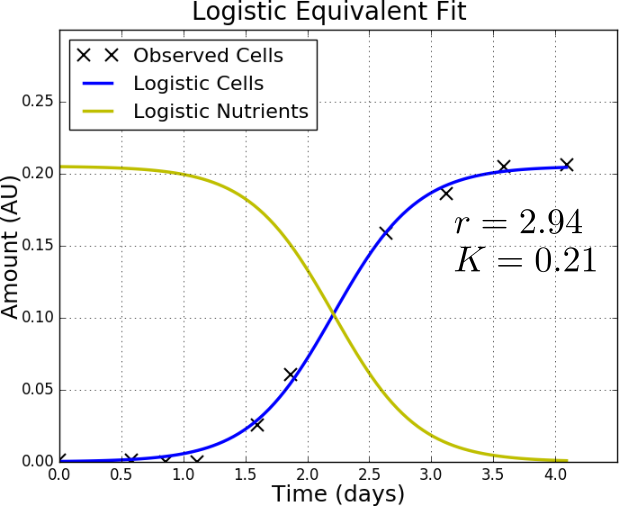
\includegraphics[width=\linewidth]{final/logistic}
  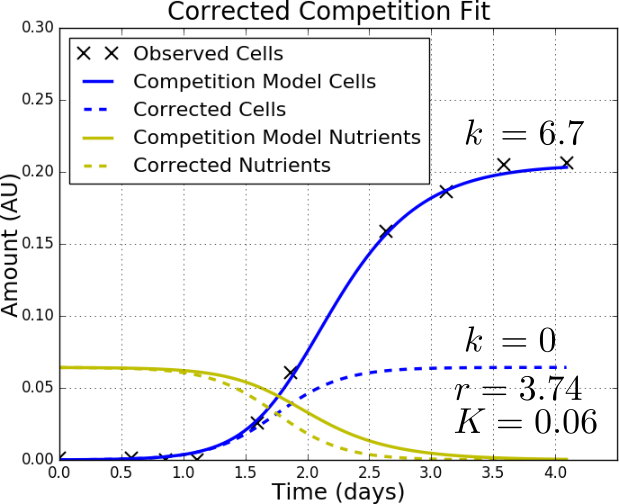
\includegraphics[width=\linewidth]{final/competition}
  \captionof{figure}{\textbf{Using the competition model to correct
      for competition.} Fits are to culture (R10, C3) of P15 which
    grew faster and reached a higher final cell density than its
    neighbours (not shown). According to the competition model, this
    is because this culture competed for more nutrients. To reach the
    same final cell density, the logistic equivalent model requires a
    higher amount of starting nutrients for this culture and a
    different amount for each neighbour. The correction to the
    competition model simulates how growth would have appeared without
    competition and allows us to return parameters \(r\) and \(K\) of
    the logistic model.}
  \label{fig:correction}
\end{Figure}


%%% Local Variables:
%%% mode: latex
%%% TeX-master: "report"
%%% End:

\subsection{\thesubsection~Making an initial guess}
\label{sec:initial_guess}

Achieving good fits of the competition model requires making a good
initial guess. To fit the competition model to small simulated zones I
could simply use many random parameter guesses. However, for fitting a
full plate with 387 parameters the chance of any random guess being
close to the ``true'' values is much smaller and more sophisticated
guessing methods are required. I did not understand the disagreement
between mass action logistic and competition model estimates of \(b\)
which is only reduced when parameters are converted to logistic model
\(r\) and \(K\) (see Section~\ref{sec:correction}). Without this
conversion fitness rankings, using \(b\), are inverted between the two
models. I instead assumed that there was a more fundamental
disagreement between models and developed the ``Imaginary Neighbour
Model'' for guessing competition model \(b\). This allowed good fits
to be made. I did not have time to compare imaginary neighbour
guessing with logistic model guessing so it is unclear which method is
better.

\subsubsection{\thesubsubsection~Guessing initial amounts}


Recall from the competition model reaction equations
(\ref{eq:reaction} and \ref{eq:diffusion_reaction}) that nutrients can
only diffuse or be converted to cells. Thus, assuming that
reactions are nearly complete at the end of cell observations and that
\(C_{t_{0}} << N_{t_{0}}\), the total initial amount of nutrients,
\(N_{Tot}\), can be estimated using,
\begin{equation}
  \label{eq:N_Tot}
  N_{Tot} = n_{I}N^{I}_{t_{0}} + n_{E}N^{E}_{t_{0}} \approx C_{F},
\end{equation}
where \(C_{F}\) is the total of final cell measurements, \(n_{I}\) and
\(n_{E}\) are the numbers of internal and edge cultures, and
\(N^{I}_{t_{0}}\) and \(N^{E}_{t_{0}}\) are initial nutrient amounts
for internal and edge cultures (see
Section~\ref{sec:fitting_comp}). Using (\ref{eq:N_Tot}) and an estimate
for the ratio of area associated with edge cultures to area associated
with internal cultures,
\(A_{r} = A^{E} / A^{I} = N^{E}_{t_{0}} / N^{I}_{t_{0}}\), I made
guesses of \(N^{I}_{t_{0}}\) and \(N^{E}_{t_{0}}\) using,
%
\begin{equation}
  \label{eq:N_0_guesses}
  \begin{aligned}
    % &A_{r} = A_{E} / A_{I} = N^{E}_{t_{0}} / N^{I}_{t_{0}}\\
    % &N_{Tot} = n_{I}N^{I}_{t_{0}} + n_{E}N^{E}_{t_{0}} \approx C_{F}\\
    &N^{I}_{t_{0}} = N_{Tot} / (n_{I} + n_{E}A_{r})\\
    &N^{E}_{t_{0}} = N_{Tot} / (n_{I}/A_{r} + n_{E}).
    % &N^{E}_{t_{0}} = (N_{Tot} - n_{I}N^{I}_{t_{0}}) / n_{E}.
  \end{aligned}
\end{equation}
%
When \(A_{r} = 1\), (\ref{eq:N_0_guesses}) reduces to the initial
nutrient guess for the one initial nutrient parameter model.
\\
In QFA using dilute cultures, \(C_{t_{0}}\) falls below the level of
detection.  I did not estimate initial guesses of \(C_{t_{0}}\) and
instead ran multiple fits over a range of \(C_{t_{0}}\) values in
logspace. What was the range?
\\
(Discussion: Recent work Herrmann and Lawless suggests that direct
measures of \(C_{t_{0}}\) may not be reliable due to heterogeneity
between inoculated cells; many inoculated cells don't grow and only
the fastest growing cells contribute significantly to the final
population.)
\subsubsection{\boldmath \thesubsubsection~Guessing  \(b\) \unboldmath}


\subsubsection{\boldmath \thesubsubsection~Guessing \({k_{n}}\) \unboldmath}


\graphicspath{{images/guessing/}}
\begin{Figure}
  \centering
  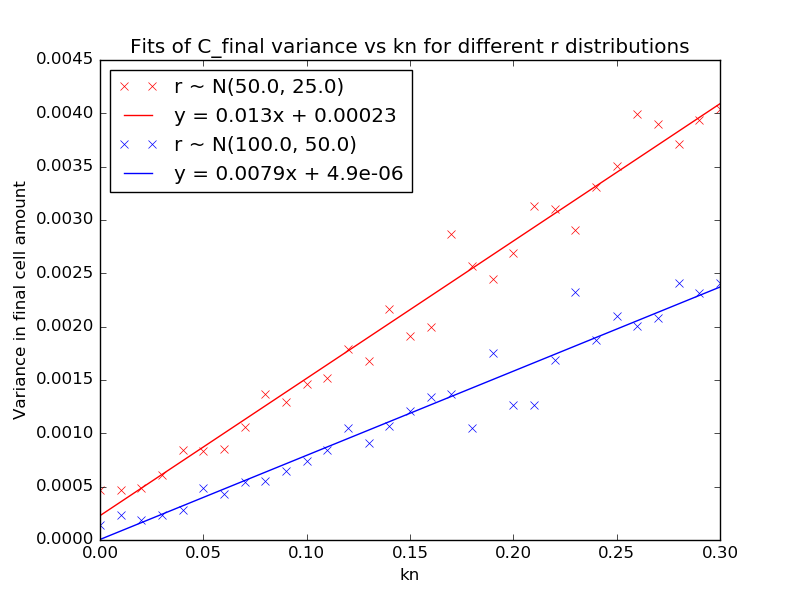
\includegraphics[width=\linewidth]{final/kn_guessing}
  \captionof{figure}{\textbf{Guessing \(\bm{k_{n}}\) from the variance in
      final cell amounts.} The competition model is simulated for a
    16x24 format plate using two random sets of culture-level \(b\)
    parameters drawn from different normal distributions. Each set of
    \(b\) parameters is simulated with a range of \(k_n\) parameter
    values. The variance in final cell density for all cultures is
    plotted against \(k_n\) for each simulation. Lines are shown for
    least squares fits to points from each set of \(b\) parameters.}
  \label{fig:kn_guessing}
\end{Figure}


\subsection{\thesubsection~Development of a genetic algorithm}
\subsection{\thesubsection~Model comparison using a single QFA plate}
\subsection{\thesubsection~Cross-plate calibration and validation}
